\documentclass[12pt,italian,a4paper,oneside,openright]{book}
\usepackage{url,amsfonts,epsfig}
\usepackage[italian]{babel}
\usepackage[utf8]{inputenc}
\usepackage[utf8]{inputenc}
\usepackage[format=hang,font=footnotesize]{caption}
\usepackage{vmargin}
\usepackage{amsmath}
\usepackage{indentfirst}
\usepackage{graphicx}
\usepackage{textcomp}
\usepackage{amssymb}
\usepackage{setspace}
\usepackage[linesnumbered,ruled,vlined]{algorithm2e}
\renewcommand{\thealgocf}{}
\usepackage[bottom]{footmisc}
\usepackage{xcolor}
\usepackage{listing}
\usepackage[chapter]{minted}
\usepackage{etoolbox}
\apptocmd{\thebibliography}{\raggedright}{}{}

\usepackage[hyperindex]{hyperref} %per l'indice interattivo
\hypersetup{colorlinks=true, linkcolor=black} %per colorare i link


\begin{document}

{
    \thispagestyle{empty}
    
    \vskip 1cm \large \centerline{\textsc{Universit\`a degli Studi di
    Napoli ``Parthenope''}}
    
    \centerline {\textsc{Dipartimento di Scienze e Tecnologie}}
    
    \centerline {\small\textsc{Corso di laurea Triennale in Informatica}}
    \vskip 0.5cm

    \begin{center}
    
\includegraphics[scale=0.8]{img/logo.eps}
    \end{center}
    
    \vskip 0.5cm
    
    \large \centering {\textsc{Algoritmi e Strutture Dati e Laboratorio di Algoritmi e Strutture Dati}}
    
    \vskip 0.5cm
    
    \centerline {Relazione progetto traccia 2}
    
    \vskip 0.5cm

    \large
    \begin{minipage}[t]{7cm}
    \textsc{Docenti}
    
    Prof. Alessio Ferone\newline
    Prof. Francesco Camastra
    
    \end{minipage}
    \hfill
    \begin{minipage}[t]{6cm}
    \hfill \textsc{Candidato}
    
    \hfill Vittorio Fones 0124/1384
    \end{minipage}
    
    \vskip 1.0 cm \Large \centerline {Anno Accademico 2019-2020}
    \vfill \eject
} % fine frontespizio

\pagenumbering{Roman}
\baselineskip 1.5em


\renewcommand\listingscaption{Codice}


\markboth{Indice}{Indice}
\tableofcontents
\listoffigures
\renewcommand*{\listlistingname}{Indice dei codici sorgente}
\listoflistings
\newpage

\pagenumbering{arabic}
\part{}
\def\baselinestretch{1}
\chapter{Albero red-black di hash table}
\def\baselinestretch{1.66}
\thispagestyle{headings}

\def\baselinestretch{1}
\section{Descrizione problema}
\def\baselinestretch{1.66}
\thispagestyle{headings}

Il problema in analisi prevede di creare una struttura dati, in C++, che d'ora in avanti chiameremo
\textbf{red-black hash}, in grado di immagazzinare delle stringhe alfanumeriche. Tale struttura
\`e l'unione di un \textbf{albero rosso-nero}, o \textbf{albero
red-black}, (albero binario di ricerca autobilanciato), e delle \textbf{tavole di hash} (array associativi usati creare mappe tra chiavi e valori): all'interno di ogni nodo di tale albero,
vi \`e presente una \textbf{hash table}, struttura dati che associa per ogni chiave un singolo valore, al cui
interno sono presenti delle stringhe. La traccia prevedeva di poter effettuare operazioni
\textbf{C.R.D.}\footnote{Create Retrieve Delete. Operazioni tipiche delle basi di dati, ma senza la
possibilit\`a di effettuare Updates.} su tuple nel formato \verb|chiave1:chiave2:stringa| . 
La chiave 1 indicizza un nodo dell'albero red black, mentre la chiave 2 viene usata per associare la stringa all'interno
della hashtable.
Vi \`e quindi una relazione \verb|1:1| per i nodi dell'albero e l'hash table, e \verb|1:M| tra l'hash table
e le stringhe, dove \textbf{M} \`e la dimensione massima dell'hash table.

\def\baselinestretch{1}
\section{Descrizione strutture dati}
\def\baselinestretch{1.66}
\thispagestyle{headings}
\subsection{Alberi binari di ricerca}
\indent Gli \textbf{alberi binari di ricerca} sono delle strutture dati
 che immagazzinano dati in un albero avente in ogni nodo due 
 figli. Gli \textbf{ABR} (o in inglese BST) godono della seguente propriet\`a:
 $\forall \ x \in \ $BST$ :\ key(x.left) \leq key(x) < key(x.right)$. 
 Ovvero ogni nodo in un ABR ha come valore della chiave un valore
 maggiore del figlio sinistro ma minore di quello destro.
 \newline Ci\`o assicura operazioni in una complessit\`a 
 \textbf{logaritmica} data dalla profondit\`a dell'albero.
 Il problema sorge nel caso in cui avvengono frequenti cancellazioni che seppur mantengono
 la propriet\`a degli ABR, degradano tale albero in una lista concatenata
 portando le operazioni di inserimento, cancellazione
 e ricerca ad avere complessit\`a lineare.

\subsection{Alberi Red-Black}
Gli alberi red black sono degli alberi binari di ricerca
\textbf{autobilancianti}. Ogni volta che si inserisce un nuovo 
nodo, o lo 
si cancella si effettuano delle operazioni per bilanciare 
l'albero. Gli alberi rosso neri posseggono \textbf{5 propriet\`a} 
utili
ai metodi di supporto $insertFix()$ e $deleteFix()$ per garantire che le complessit\`a
peggiori abbiano al pi\`u come valore l'altezza dell'albero, ovvero $O(log_2n)$. 
I metodi di supporto all'inserimento e alla cancellazione fanno uso delle rotazioni di un nodo,
operazione che permette di compattare l'albero e garantirne il corretto bilanciamento.
Di seguito verranno elencate tali propriet\`a:
\begin{itemize}
    \item ogni nodo \`e rosso o nero;
    \item la radice \`e nera;
    \item ogni foglia \`e nera;
    \item se un nodo \`e rosso, allora entrambi i suoi figli sono neri;
    \item per ogni nodo, tutti i cammini semplici che vanno dal nodo alle foglie sue discendenti
    contengono lo stesso numero di nodi neri.
\end{itemize}

\subsection{Hash Table ad indirizzamento aperto}
Le \textbf{Hash Table}, o hash map, sono delle strutture dati che permettono di associare ad una
chiave un singolo valore. Quando si vuole memorizzare un dato
si usa la sua chiave e vi si applica una \textbf{funzione di hashing} che ne calcoler\`a un indice usato per inserire nell'array tale dato. Pu\`o capitare per\`o che una funzione hash applicata su chiavi diverse 
indicizzi celle simili dell'array, per tanto bisogna gestire queste \textit{collisioni}.
La tecnica usata per risolvere le collisioni \`e del tipo a \textbf{indirizzamento aperto}, ovvero non facendo
uso dei puntatori si \textit{ispeziona} l'hashtable fino a incontrare una posizione libera,
se presente. Il metodo di ispezione scelto \`e quello del \textbf{doppio hashing}: rispetto
ad altre ispezioni, quella del doppio hashing trova una posizione in modo pi\`u veloce.
Nei capitoli successivi vedremo nel dettaglio il funzionamento.
\newpage
\def\baselinestretch{1}
\section{Formato di input e di output}
\def\baselinestretch{1.66}
\thispagestyle{headings}

\subsection{Input}
\indent Il programma lavora su tuple nel formato $chiave1:chiave2:stringa$ e i dati in input sono dati da:
\begin{itemize}
    \item file di testo da selezionare all'avvio contenente le tuple;
    \begin{lstlisting}[language=bash]
    $ ./rbhash inputs/asd.txt
    \end{lstlisting}
    \item opzione da tastiera per effettuare operazioni sulle tuple.
     \begin{lstlisting}[language=bash]
    >_ 1:2:stringa
    \end{lstlisting}
\end{itemize}
Il programma legger\`a le righe e allocher\`a nodi e hashtable in base alle chiavi date in input.
\subsection{Output}
L'output del programma \`e un menu contestuale in cui l'utente pu\`o effettuare le operazioni
mostrate di seguito:


\begin{lstlisting}[language=bash]
  **** MENU ****

   1. Insert
   2. Remove
   3. Query
   4. Print
   0. Exit
  >_
\end{lstlisting}


\noindent Tutte le opzioni restituiscono un output di avvenuta operazione con dettagli su eventuali errori,
ad eccezzione della stampa (opzione 4) che restituisce in output l'intera struttura dati caricata
in memoria.\newpage
\def\baselinestretch{1}
\section{Descrizione algoritmo}
\def\baselinestretch{1.66}
\thispagestyle{headings}
\subsection{Pseudo codice}

\textbf{L'insertimento} nella struttura dati creata va effettuare prima una ricerca
del nodo di chiave $key1$. Se dovesse riscontrare un esito negativo si procede
alla allocazione di un hashtable e un nuovo nodo. In caso contrario si procede alla ricerca
di una cella della tavola di hash con la $key2$, se anche questa ricerca restituisce un esito
negativo allora si procede con l'inserimento.

\BlankLine
\IncMargin{1.5em}
\begin{algorithm}[H]
\setstretch{1.1}
\caption{Insert}
\SetKwData{Left}{left}\SetKwData{This}{this}\SetKwData{Up}{up}
\SetKwFunction{Union}{Union}\SetKwFunction{FindCompress}{FindCompress}
\SetKwInOut{Input}{input}\SetKwInOut{Result}{result}
\SetKwIF{If}{ElseIf}{Else}{if}{:}{elif}{else:}{}
\Input{ key1, key2, string }
\Result{ $true$ if successfull, $false$ if not }
\emph{$node$ = Search in Red Black with $key1$}\;
\If{$\nexists \ node$} {
    \emph{new Hashtable()}\;
    \emph{new Node()}\;
    \emph{Hashtable.insert(key2, string)}\;
    \emph{Node.insert(key1, Hashtable)}\;
    return \emph{true}\;
}
\Else{\If{$\nexists \ node.Hashtable.search(key2)$} {
        \emph{node.Hashtable.insert(key2, d)}\;
        return \emph{true}\; }}
return \emph{false}\;
\end{algorithm}

\indent La \textbf{ricerca} controlla la correttezza delle chiavi e della stringa inserita nella tupla:
in caso di riscontro positivo la function ritorner\`a il nodo dell'albero. Questo comportamento \`e stato previsto
per poter evitare di effettuare una o pi\`u ricerche nella
procedura di cancellazione.

\BlankLine
\IncMargin{1.5em}
\begin{algorithm}[H]
\setstretch{1.1}
\caption{Search (retrieve) }
\SetKwData{Left}{left}\SetKwData{This}{this}\SetKwData{Up}{up}
\SetKwFunction{Union}{Union}\SetKwFunction{FindCompress}{FindCompress}
\SetKwInOut{Input}{input}\SetKwInOut{Result}{result}
\SetKwIF{If}{ElseIf}{Else}{if}{:}{elif}{else:}{}
\Input{ key1, key2, string }
\Result{node if found $or$ NIL if not found}
\emph{$node$ = Search in Red Black with $key1$}\;
\If{$\exists \ node$} {
    \emph{$data$ = node.Hashtable.search(key2)}\;
    \If{string = data } {
        return \emph{node}\;
    }
}
return \emph{NIL}\;
\end{algorithm}
\newpage
\indent La \textbf{cancellazione} di una tupla effettua una operazione di ricerca nella struttura dati.
Se la ricerca ha risconto positivo allora si procede con i due casi della rimozione:
se la chiave secondaria indicizza una hashtable in cui vi \`e presente un solo elemento, allora
si canceller\`a l'intero nodo red black, altrimenti si procede alla normale rimozione dalla hashtable.
\BlankLine
\IncMargin{1.5em}
\begin{algorithm}[H]
\setstretch{1.1}
\caption{Remove (delete)}
\SetKwData{Left}{left}\SetKwData{This}{this}\SetKwData{Up}{up}
\SetKwFunction{Union}{Union}\SetKwFunction{FindCompress}{FindCompress}
\SetKwInOut{Input}{input}\SetKwInOut{Result}{result}
\SetKwIF{If}{ElseIf}{Else}{if}{:}{elif}{else:}{}
\Input{ key1, key2, string }
\Result{true if deleted $or$ false if not}
\emph{node = Search in Red Black Hash}\;
\If{$node \neq NIL$} {
    \eIf{node.Hashtable.capacity = 1} {
    \emph{delete node}\;}
    {node.Hashtable.remove(key2)\;}
    return \emph{true}\;}
return \emph{false}\;
\end{algorithm}

\subsection{Diagrammi delle classe e dettagli architetturali}
\subsubsection{Nodi Binari}
\indent I nodi facenti parti degli alberi
binari sono nodi che derivano da una classe astratta che a sua
volta estende un nodo generico.\newline
\indent Per permettere agli alberi binari di usare come parametro
templato un generico nodo, si \`e sfruttato un particolare
pattern strutturale chiamato \textbf{CRTP} \textit{(Curiously recurring 
template pattern)}: una classe (e.g. ConcreteBinaryNode) eredita
da una classe astratta che usa il CRTP (e.g. AbstractBinaryNode ha come parametro templato un generico nodo), usando
come parametro di specializzazione se stessa. Il nodo concreto
RedBlack in pi\`u implementa la classe color. Si \`e scelta tale tecnica che non porta
miglioramenti sostanziali al codice se non quella di nascondere
dettagli implementativi e un' indipendenza dalla rappresentazione in memoria del colore.
\begin{center}
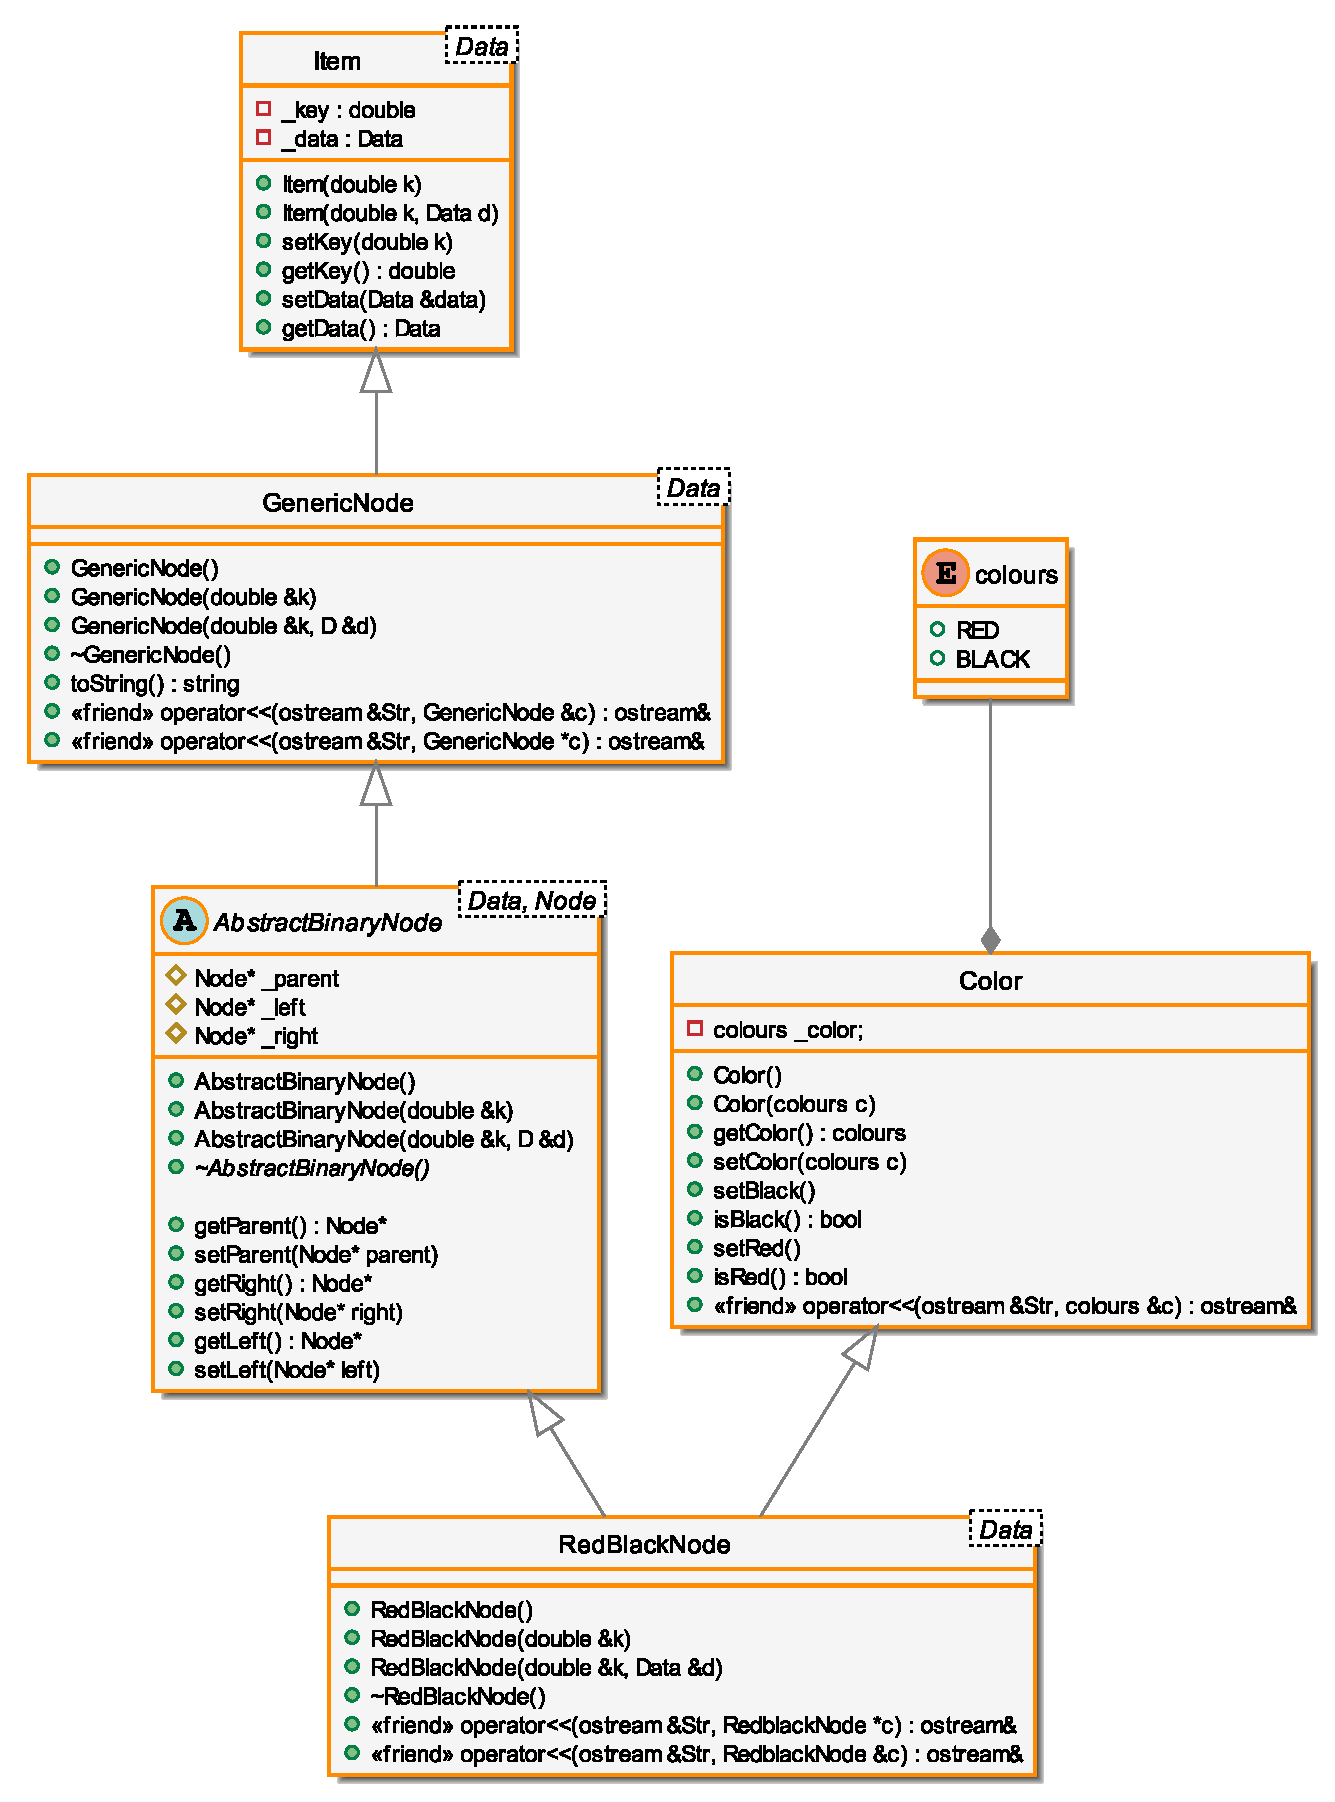
\includegraphics[scale=0.6]{src/rbhash/2img/nodes.eps}
\captionof{figure}{Nodi degli alberi}
\end{center}
\subsubsection{Alberi}
Un albero Rosso Nero \`e un albero binario di ricerca auto
bilanciante, per tanto si \`e scelto di estendere la classe
BinarySearchTree ed aggiungere i metodi di supporto al bilanciamento. Inoltre due metodi virtuali (insert e delete), sono
stati ridefiniti nell'implementazione del Red Black.
\textit{$insertNode()$} nella class RedBlackTree richiama tramite scope la insert
di BinarySearchTree e successivamente applica il
\textbf{fix} dei red black.
\begin{center}
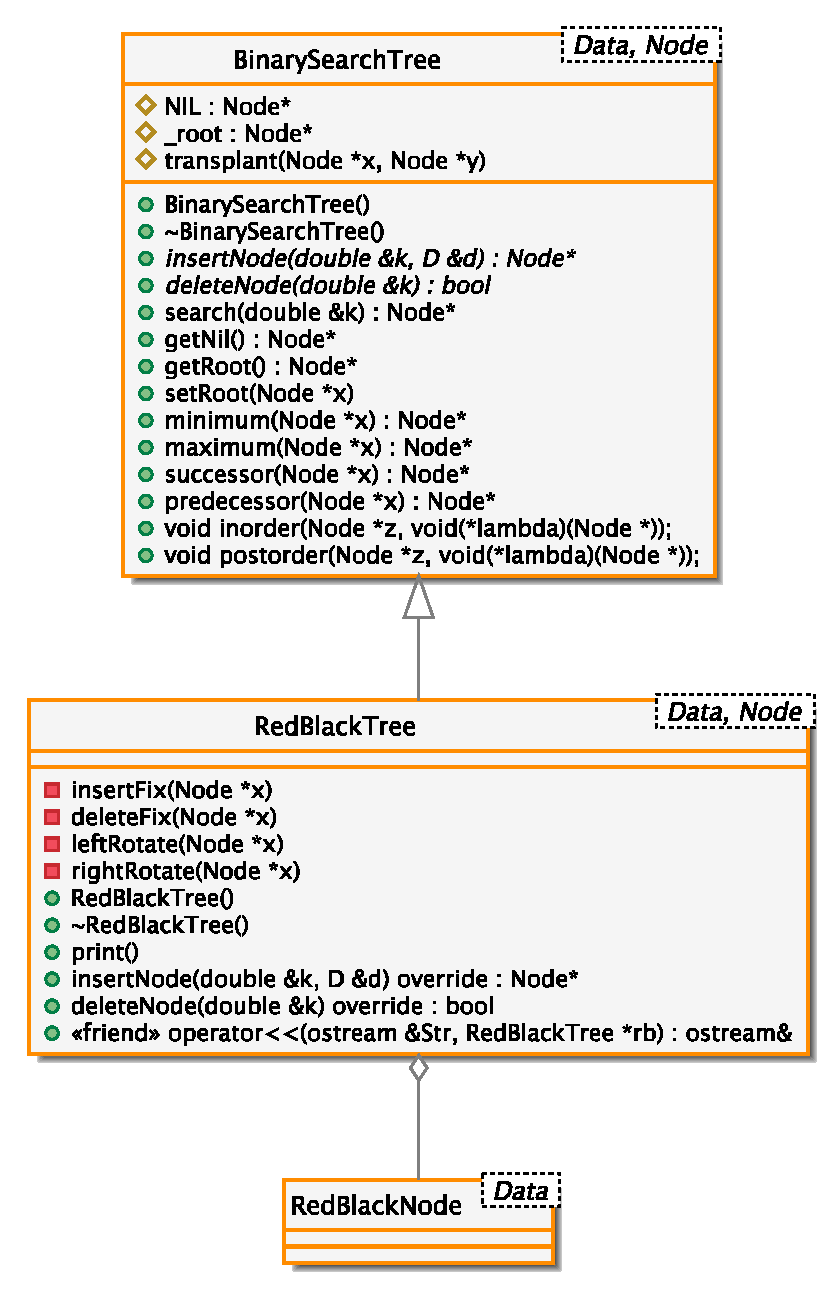
\includegraphics[scale=0.7]{src/rbhash/2img/trees.eps}
\captionof{figure}{Alberi}
\end{center}
\subsection{Hash Table}
Onde evitare di dover riscrivere codice si \`e scelto di sfruttare
il nodo generico anche per l'\textbf{HashTable}. A tal proposito
si \`e sviluppato una tabella hash ad \textbf{indirizzamento aperto} che
prende in input come paramentro templato, il dato da conservare.
Per risolvere le collisioni si \`e scelto di usare due funzioni hash:
\texttt{k} \`e un valore double che indica
la chiave, $\texttt{i}$ \`e l'iteratore che al massimo 
$\texttt{m}$ volte \footnote{m \`e il size dell'hashtable}  
applicher\`a la funzione di hash. La prima restituisce un indice con valore compreso
tra $[0, m]$, mentre la seconda funzione di hash un valore compreso tra $[1, m-1]$. 
Verr\`a usata la prima funzione di hash e in caso di collisione
si riapplicher\`a
$h(i, m) = (h_1(k) + i * h_2(k)) \ mod \ m$. Sebbene con un costo 
computazionale pi\`u alto, il doppio hashing risolve le collisioni
pi\`u in fretta rispetto allispezione lineare o quadratica.\newline \indent 
La funzione $search()$ nella class \textbf{HashTable}
\`e stata sovraccaricata per restituire valori diversi. Con la 
ricerca per valore si restituise, se disponibile un indice che 
usato nella seconda funzione di ricerca restituisce il dato.

\begin{center}
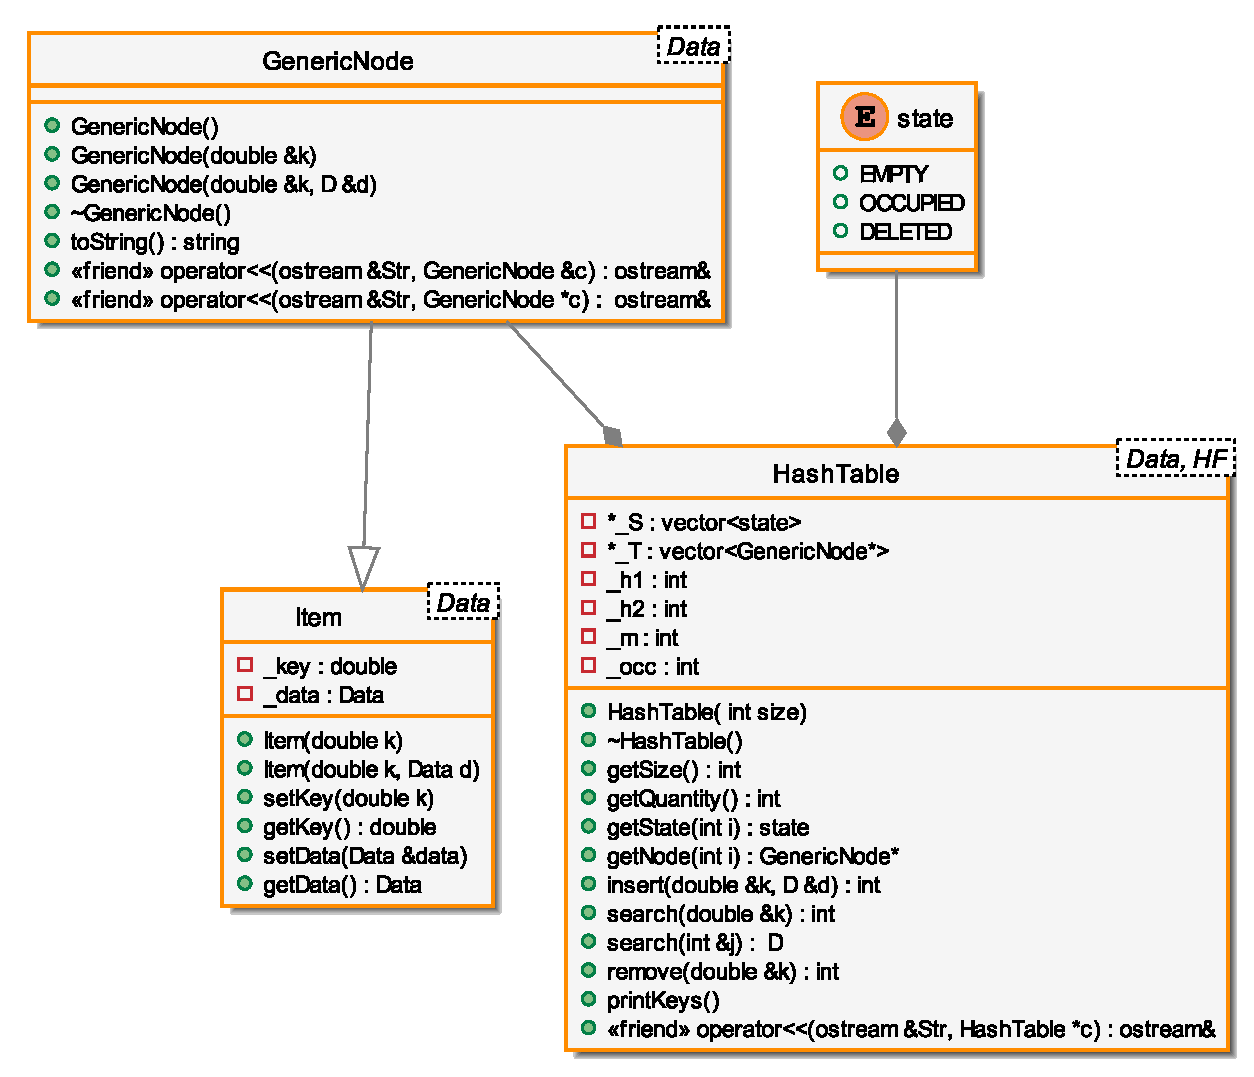
\includegraphics[scale=0.7]{src/rbhash/2img/hash.eps}
\captionof{figure}{Hash Table}
\end{center}

\newpage
\subsection{Red Black Hash}
La struttura dati realizzata fa uso degli alberi red black
e delle tavole di hash come spiegato nel primo paragrafo.
Si è scelto di usare una classe \textbf{Parser} per riempire la
struttura dati delle tuple contenute nel file di testo
o di quelle inserite tramite riga di comando.
\begin{center}
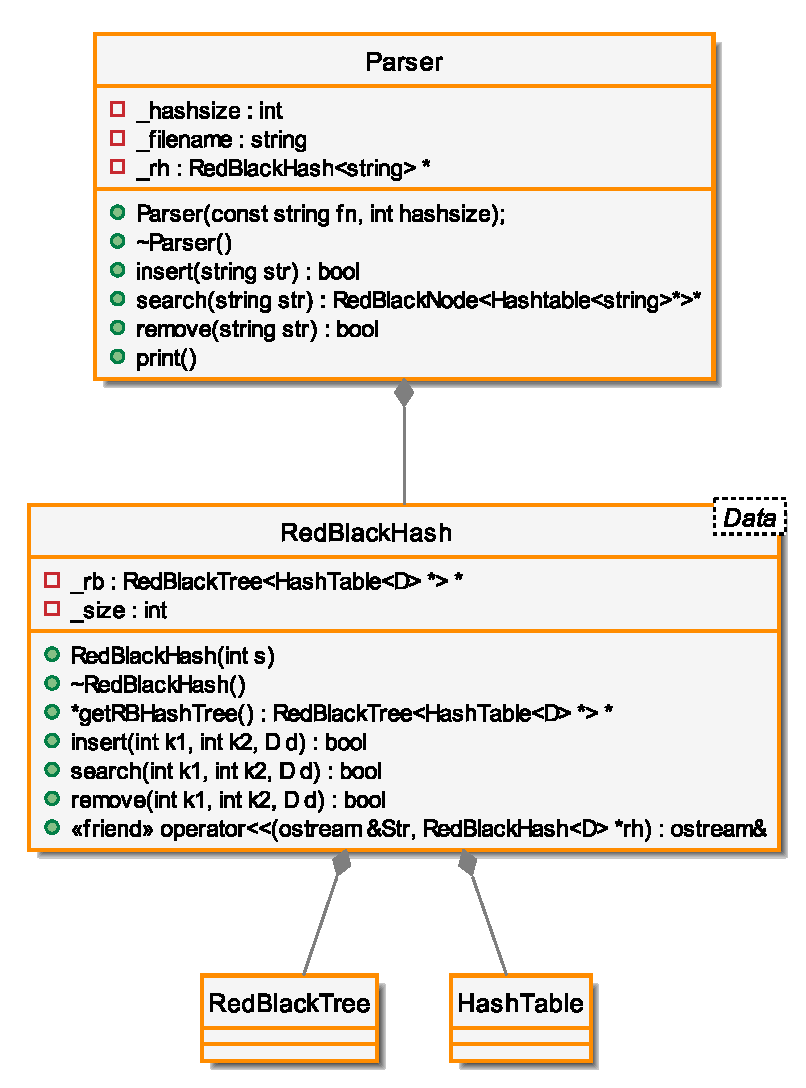
\includegraphics[scale=0.8]{src/rbhash/2img/rbhash.eps}
\captionof{figure}{Parser e RBH}
\end{center}\newpage
\def\baselinestretch{1}
\section{Studio complessit\`a}
\def\baselinestretch{1.66}
\thispagestyle{headings}
\indent Come detto precedentemente gli alberi Red Black hanno una complessit\`a temporale
nel \textbf{caso peggiore} al pi\`u equivalente ad $O(log_2 n)$ poich\'e bisogna scorrere tutto
l'albero in profondit\`a.\newline

\indent Le tabelle di hash a indirizzamento aperto, con doppia funzione di hash hanno complessit\`a temporali
prossime all'\textit{hashing 'ideale'}. Per poter assicurare che le due funzioni di hash producano
complessit\`a nel caso medio uguali a $O(1)$, si deve scegliere un valore della tavola di hash uguale ad
un numero primo o come potenza di due, e usare la seconda funzione di hash (quella che scandisce l'offset
dato dalle ispezioni successive) con un valore poco pi\`u piccolo di $m$ ($m-1$ o $m-2$).
In tal modo il doppio hashing usa $O(m^2)$ sequenze di ispezione,
perch\'e ogni coppia ($h_1(k), h_2(k)$) produce una distinta sequenza di ispezione.
Le \textbf{hashtable nel caso migliore}, ovvero non avendo nessuna collisione inseriscono,
cercano e cancellano i dati in $O(1)$.
Nel caso \textbf{peggiore} avremo un tempo massimo di $O(m)$,
dovuto alla scansione lineare di tutta la tavola di hash: ci\`o \`e  dovuto alla hashtable che si riempie
cio\`e quando il \textbf{ fattore di carico} (rapporto di elementi
inseriti e size della tavola) $\alpha$ tende a $1$.\newline

\indent Nella struttura dati \textbf{red-black hash} quando effettuiamo un \textbf{inserimento} andremo prima
ad effettuare una ricerca nell'albero rosso nero ($O(log_2n)$):
\begin{itemize}
    \item se esiste il nodo di chiave 1 allora
effettuiamo una ricerca nell'hash table tramite la chiave 2, e se possibile concludiamo l'inserimento.
Nel caso medio avremo una complessit\`a del tipo
$O(log_2n) + O(1) + O(1)$ e $O(log_2n) + O(m) + O(m)$ se l'hashtable ha un fattore di carico prossimo
all'1. In altri termini $\mathbf{O(log_2n)}$ e $\mathbf{O(m+log_2n)}$.;
    \item se invece il nodo di chiave 1 non esiste, dobbiamo allocare una hashtable, mappare la stringa alla chiave 2
e inserirla nell'albero: ci\`o porta una complessit\`a pari a $O(log_2n) + O(1) +  O(log_2n)$ ovvero 
$\mathbf{O(log_2n)}$.
\end{itemize}
L'operazione di \textbf{ricerca} impiega $\mathbf{O(m+log_2n)}$ nel caso in cui esista il nodo
con chiave 1 e la ricerca nella tavola hash restituisca l'indice in un tempo lineare; l'uso di tale indice 
serve per accedere al dato in $O(1)$. Nel caso migliore invece la ricerca avviene in
$\mathbf{O(log_2n)}$.\newline
La \textbf{cancellazione} ha complessit\`a uguali alle precendenti: si effettua una ricerca e
se l'hashtable ha solo un elemento allora si provvede a cancellare l'intero nodo dall'albero, altrimenti
si cancella solamente nell'hashtable: pertanto $\mathbf{O(log_2n)}$ oppure $\mathbf{O(m+log_2n)}$.
\newline
Tramite questo prospetto possiamo affermare che i casi peggiori sono dettati dalla tavola di hash e dipende
tutto dal suo fattore di carico.
\def\baselinestretch{1}
\section{Test e risultati}
\def\baselinestretch{1.66}
\thispagestyle{headings}

\subsection{Test effettuati}\newpage
\def\baselinestretch{1}
\section{Codice sorgente}
\def\baselinestretch{1.66}
\thispagestyle{headings}

\inputminted
[fontsize=\small,baselinestretch=1,
frame=lines,
framesep=10pt,
linenos=true,tabsize=2,
breaklines=true]{c++}{tesina_tex/source/graph/heap.hpp}
\inputminted
[fontsize=\small,baselinestretch=1,
frame=lines,
framesep=10pt,
linenos=true,tabsize=2,
breaklines=true]{c++}{tesina_tex/source/graph/heap.cpp}

\newpage
\inputminted
[fontsize=\small,baselinestretch=1,
frame=lines,
framesep=10pt,
linenos=true,tabsize=2,
breaklines=true]{c++}{tesina_tex/source/graph/minHeap.hpp}
\inputminted
[fontsize=\small,baselinestretch=1,
frame=lines,
framesep=10pt,
linenos=true,tabsize=2,
breaklines=true]{c++}{tesina_tex/source/graph/minHeap.cpp}
\newpage
\inputminted
[fontsize=\small,baselinestretch=1,
frame=lines,
framesep=10pt,
linenos=true,tabsize=2,
breaklines=true]{c++}{tesina_tex/source/graph/minPriorityQueue.hpp}
\inputminted
[fontsize=\small,baselinestretch=1,
frame=lines,
framesep=10pt,
linenos=true,tabsize=2,
breaklines=true]{c++}{tesina_tex/source/graph/minPriorityQueue.cpp}
\newpage


\inputminted
[fontsize=\small,baselinestretch=1,
frame=lines,
framesep=10pt,
linenos=true,tabsize=2,
breaklines=true]{c++}{tesina_tex/source/graph/galacticgraph.hpp}
\inputminted
[fontsize=\small,baselinestretch=1,
frame=lines,
framesep=10pt,
linenos=true,tabsize=2,
breaklines=true]{c++}{tesina_tex/source/graph/galacticgraph.cpp}
\newpage

\inputminted
[fontsize=\small,baselinestretch=1,
frame=lines,
framesep=10pt,
linenos=true,tabsize=2,
breaklines=true]{c++}{tesina_tex/source/graph/loader.hpp}
\inputminted
[fontsize=\small,baselinestretch=1,
frame=lines,
framesep=10pt,
linenos=true,tabsize=2,
breaklines=true]{c++}{tesina_tex/source/graph/loader.cpp}
\newpage

\inputminted
[fontsize=\small,baselinestretch=1,
frame=lines,
framesep=10pt,
linenos=true,tabsize=2,
breaklines=true]{c++}{tesina_tex/source/graph/debug.hpp}
\inputminted
[fontsize=\small,baselinestretch=1,
frame=lines,
framesep=10pt,
linenos=true,tabsize=2,
breaklines=true]{c++}{tesina_tex/source/graph/item.hpp}
\newpage

\inputminted
[fontsize=\small,baselinestretch=1,
frame=lines,
framesep=10pt,
linenos=true,tabsize=2,
breaklines=true]{c++}{tesina_tex/source/graph/vertex.hpp}
\inputminted
[fontsize=\small,baselinestretch=1,
frame=lines,
framesep=10pt,
linenos=true,tabsize=2,
breaklines=true]{c++}{tesina_tex/source/graph/vertex.cpp}
\newpage

\inputminted
[fontsize=\small,baselinestretch=1,
frame=lines,
framesep=10pt,
linenos=true,tabsize=2,
breaklines=true]{c++}{tesina_tex/source/graph/graph.hpp}
\inputminted
[fontsize=\small,baselinestretch=1,
frame=lines,
framesep=10pt,
linenos=true,tabsize=2,
breaklines=true]{c++}{tesina_tex/source/graph/graph.cpp}
\newpage\newpage

\part{}
\def\baselinestretch{1}
\chapter{Albero red-black di hash table}
\def\baselinestretch{1.66}
\thispagestyle{headings}

\def\baselinestretch{1}
\section{Descrizione problema}
\def\baselinestretch{1.66}
\thispagestyle{headings}

Il problema in analisi prevede di creare una struttura dati, in C++, che d'ora in avanti chiameremo
\textbf{red-black hash}, in grado di immagazzinare delle stringhe alfanumeriche. Tale struttura
\`e l'unione di un \textbf{albero rosso-nero}, o \textbf{albero
red-black}, (albero binario di ricerca autobilanciato), e delle \textbf{tavole di hash} (array associativi usati creare mappe tra chiavi e valori): all'interno di ogni nodo di tale albero,
vi \`e presente una \textbf{hash table}, struttura dati che associa per ogni chiave un singolo valore, al cui
interno sono presenti delle stringhe. La traccia prevedeva di poter effettuare operazioni
\textbf{C.R.D.}\footnote{Create Retrieve Delete. Operazioni tipiche delle basi di dati, ma senza la
possibilit\`a di effettuare Updates.} su tuple nel formato \verb|chiave1:chiave2:stringa| . 
La chiave 1 indicizza un nodo dell'albero red black, mentre la chiave 2 viene usata per associare la stringa all'interno
della hashtable.
Vi \`e quindi una relazione \verb|1:1| per i nodi dell'albero e l'hash table, e \verb|1:M| tra l'hash table
e le stringhe, dove \textbf{M} \`e la dimensione massima dell'hash table.

\def\baselinestretch{1}
\section{Descrizione strutture dati}
\def\baselinestretch{1.66}
\thispagestyle{headings}
\subsection{Alberi binari di ricerca}
\indent Gli \textbf{alberi binari di ricerca} sono delle strutture dati
 che immagazzinano dati in un albero avente in ogni nodo due 
 figli. Gli \textbf{ABR} (o in inglese BST) godono della seguente propriet\`a:
 $\forall \ x \in \ $BST$ :\ key(x.left) \leq key(x) < key(x.right)$. 
 Ovvero ogni nodo in un ABR ha come valore della chiave un valore
 maggiore del figlio sinistro ma minore di quello destro.
 \newline Ci\`o assicura operazioni in una complessit\`a 
 \textbf{logaritmica} data dalla profondit\`a dell'albero.
 Il problema sorge nel caso in cui avvengono frequenti cancellazioni che seppur mantengono
 la propriet\`a degli ABR, degradano tale albero in una lista concatenata
 portando le operazioni di inserimento, cancellazione
 e ricerca ad avere complessit\`a lineare.

\subsection{Alberi Red-Black}
Gli alberi red black sono degli alberi binari di ricerca
\textbf{autobilancianti}. Ogni volta che si inserisce un nuovo 
nodo, o lo 
si cancella si effettuano delle operazioni per bilanciare 
l'albero. Gli alberi rosso neri posseggono \textbf{5 propriet\`a} 
utili
ai metodi di supporto $insertFix()$ e $deleteFix()$ per garantire che le complessit\`a
peggiori abbiano al pi\`u come valore l'altezza dell'albero, ovvero $O(log_2n)$. 
I metodi di supporto all'inserimento e alla cancellazione fanno uso delle rotazioni di un nodo,
operazione che permette di compattare l'albero e garantirne il corretto bilanciamento.
Di seguito verranno elencate tali propriet\`a:
\begin{itemize}
    \item ogni nodo \`e rosso o nero;
    \item la radice \`e nera;
    \item ogni foglia \`e nera;
    \item se un nodo \`e rosso, allora entrambi i suoi figli sono neri;
    \item per ogni nodo, tutti i cammini semplici che vanno dal nodo alle foglie sue discendenti
    contengono lo stesso numero di nodi neri.
\end{itemize}

\subsection{Hash Table ad indirizzamento aperto}
Le \textbf{Hash Table}, o hash map, sono delle strutture dati che permettono di associare ad una
chiave un singolo valore. Quando si vuole memorizzare un dato
si usa la sua chiave e vi si applica una \textbf{funzione di hashing} che ne calcoler\`a un indice usato per inserire nell'array tale dato. Pu\`o capitare per\`o che una funzione hash applicata su chiavi diverse 
indicizzi celle simili dell'array, per tanto bisogna gestire queste \textit{collisioni}.
La tecnica usata per risolvere le collisioni \`e del tipo a \textbf{indirizzamento aperto}, ovvero non facendo
uso dei puntatori si \textit{ispeziona} l'hashtable fino a incontrare una posizione libera,
se presente. Il metodo di ispezione scelto \`e quello del \textbf{doppio hashing}: rispetto
ad altre ispezioni, quella del doppio hashing trova una posizione in modo pi\`u veloce.
Nei capitoli successivi vedremo nel dettaglio il funzionamento.
\newpage
\def\baselinestretch{1}
\section{Formato di input e di output}
\def\baselinestretch{1.66}
\thispagestyle{headings}

\subsection{Input}
\indent Il programma lavora su tuple nel formato $chiave1:chiave2:stringa$ e i dati in input sono dati da:
\begin{itemize}
    \item file di testo da selezionare all'avvio contenente le tuple;
    \begin{lstlisting}[language=bash]
    $ ./rbhash inputs/asd.txt
    \end{lstlisting}
    \item opzione da tastiera per effettuare operazioni sulle tuple.
     \begin{lstlisting}[language=bash]
    >_ 1:2:stringa
    \end{lstlisting}
\end{itemize}
Il programma legger\`a le righe e allocher\`a nodi e hashtable in base alle chiavi date in input.
\subsection{Output}
L'output del programma \`e un menu contestuale in cui l'utente pu\`o effettuare le operazioni
mostrate di seguito:


\begin{lstlisting}[language=bash]
  **** MENU ****

   1. Insert
   2. Remove
   3. Query
   4. Print
   0. Exit
  >_
\end{lstlisting}


\noindent Tutte le opzioni restituiscono un output di avvenuta operazione con dettagli su eventuali errori,
ad eccezzione della stampa (opzione 4) che restituisce in output l'intera struttura dati caricata
in memoria.\newpage
\def\baselinestretch{1}
\section{Descrizione algoritmo}
\def\baselinestretch{1.66}
\thispagestyle{headings}
\subsection{Pseudo codice}

\textbf{L'insertimento} nella struttura dati creata va effettuare prima una ricerca
del nodo di chiave $key1$. Se dovesse riscontrare un esito negativo si procede
alla allocazione di un hashtable e un nuovo nodo. In caso contrario si procede alla ricerca
di una cella della tavola di hash con la $key2$, se anche questa ricerca restituisce un esito
negativo allora si procede con l'inserimento.

\BlankLine
\IncMargin{1.5em}
\begin{algorithm}[H]
\setstretch{1.1}
\caption{Insert}
\SetKwData{Left}{left}\SetKwData{This}{this}\SetKwData{Up}{up}
\SetKwFunction{Union}{Union}\SetKwFunction{FindCompress}{FindCompress}
\SetKwInOut{Input}{input}\SetKwInOut{Result}{result}
\SetKwIF{If}{ElseIf}{Else}{if}{:}{elif}{else:}{}
\Input{ key1, key2, string }
\Result{ $true$ if successfull, $false$ if not }
\emph{$node$ = Search in Red Black with $key1$}\;
\If{$\nexists \ node$} {
    \emph{new Hashtable()}\;
    \emph{new Node()}\;
    \emph{Hashtable.insert(key2, string)}\;
    \emph{Node.insert(key1, Hashtable)}\;
    return \emph{true}\;
}
\Else{\If{$\nexists \ node.Hashtable.search(key2)$} {
        \emph{node.Hashtable.insert(key2, d)}\;
        return \emph{true}\; }}
return \emph{false}\;
\end{algorithm}

\indent La \textbf{ricerca} controlla la correttezza delle chiavi e della stringa inserita nella tupla:
in caso di riscontro positivo la function ritorner\`a il nodo dell'albero. Questo comportamento \`e stato previsto
per poter evitare di effettuare una o pi\`u ricerche nella
procedura di cancellazione.

\BlankLine
\IncMargin{1.5em}
\begin{algorithm}[H]
\setstretch{1.1}
\caption{Search (retrieve) }
\SetKwData{Left}{left}\SetKwData{This}{this}\SetKwData{Up}{up}
\SetKwFunction{Union}{Union}\SetKwFunction{FindCompress}{FindCompress}
\SetKwInOut{Input}{input}\SetKwInOut{Result}{result}
\SetKwIF{If}{ElseIf}{Else}{if}{:}{elif}{else:}{}
\Input{ key1, key2, string }
\Result{node if found $or$ NIL if not found}
\emph{$node$ = Search in Red Black with $key1$}\;
\If{$\exists \ node$} {
    \emph{$data$ = node.Hashtable.search(key2)}\;
    \If{string = data } {
        return \emph{node}\;
    }
}
return \emph{NIL}\;
\end{algorithm}
\newpage
\indent La \textbf{cancellazione} di una tupla effettua una operazione di ricerca nella struttura dati.
Se la ricerca ha risconto positivo allora si procede con i due casi della rimozione:
se la chiave secondaria indicizza una hashtable in cui vi \`e presente un solo elemento, allora
si canceller\`a l'intero nodo red black, altrimenti si procede alla normale rimozione dalla hashtable.
\BlankLine
\IncMargin{1.5em}
\begin{algorithm}[H]
\setstretch{1.1}
\caption{Remove (delete)}
\SetKwData{Left}{left}\SetKwData{This}{this}\SetKwData{Up}{up}
\SetKwFunction{Union}{Union}\SetKwFunction{FindCompress}{FindCompress}
\SetKwInOut{Input}{input}\SetKwInOut{Result}{result}
\SetKwIF{If}{ElseIf}{Else}{if}{:}{elif}{else:}{}
\Input{ key1, key2, string }
\Result{true if deleted $or$ false if not}
\emph{node = Search in Red Black Hash}\;
\If{$node \neq NIL$} {
    \eIf{node.Hashtable.capacity = 1} {
    \emph{delete node}\;}
    {node.Hashtable.remove(key2)\;}
    return \emph{true}\;}
return \emph{false}\;
\end{algorithm}

\subsection{Diagrammi delle classe e dettagli architetturali}
\subsubsection{Nodi Binari}
\indent I nodi facenti parti degli alberi
binari sono nodi che derivano da una classe astratta che a sua
volta estende un nodo generico.\newline
\indent Per permettere agli alberi binari di usare come parametro
templato un generico nodo, si \`e sfruttato un particolare
pattern strutturale chiamato \textbf{CRTP} \textit{(Curiously recurring 
template pattern)}: una classe (e.g. ConcreteBinaryNode) eredita
da una classe astratta che usa il CRTP (e.g. AbstractBinaryNode ha come parametro templato un generico nodo), usando
come parametro di specializzazione se stessa. Il nodo concreto
RedBlack in pi\`u implementa la classe color. Si \`e scelta tale tecnica che non porta
miglioramenti sostanziali al codice se non quella di nascondere
dettagli implementativi e un' indipendenza dalla rappresentazione in memoria del colore.
\begin{center}
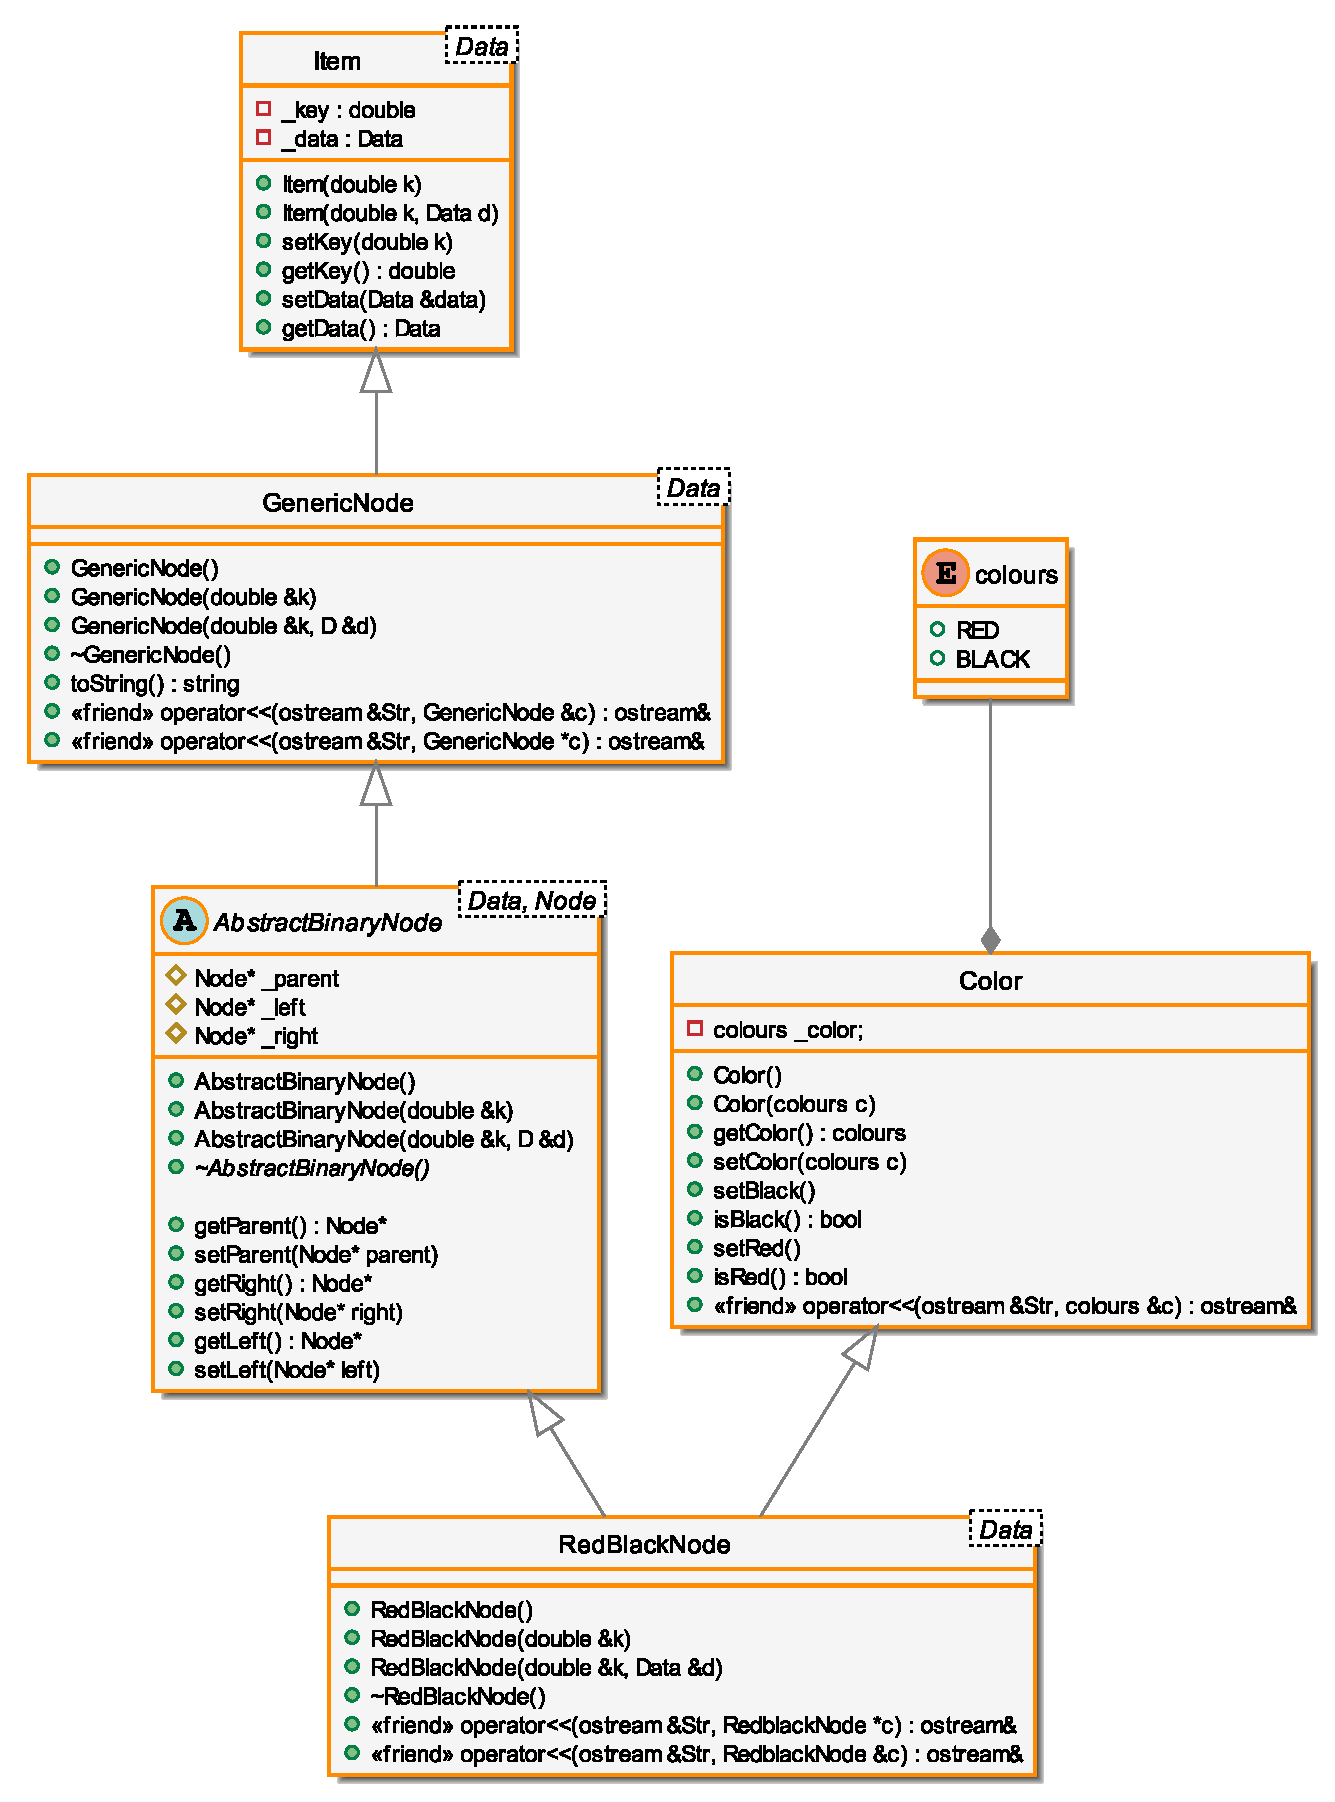
\includegraphics[scale=0.6]{src/rbhash/2img/nodes.eps}
\captionof{figure}{Nodi degli alberi}
\end{center}
\subsubsection{Alberi}
Un albero Rosso Nero \`e un albero binario di ricerca auto
bilanciante, per tanto si \`e scelto di estendere la classe
BinarySearchTree ed aggiungere i metodi di supporto al bilanciamento. Inoltre due metodi virtuali (insert e delete), sono
stati ridefiniti nell'implementazione del Red Black.
\textit{$insertNode()$} nella class RedBlackTree richiama tramite scope la insert
di BinarySearchTree e successivamente applica il
\textbf{fix} dei red black.
\begin{center}
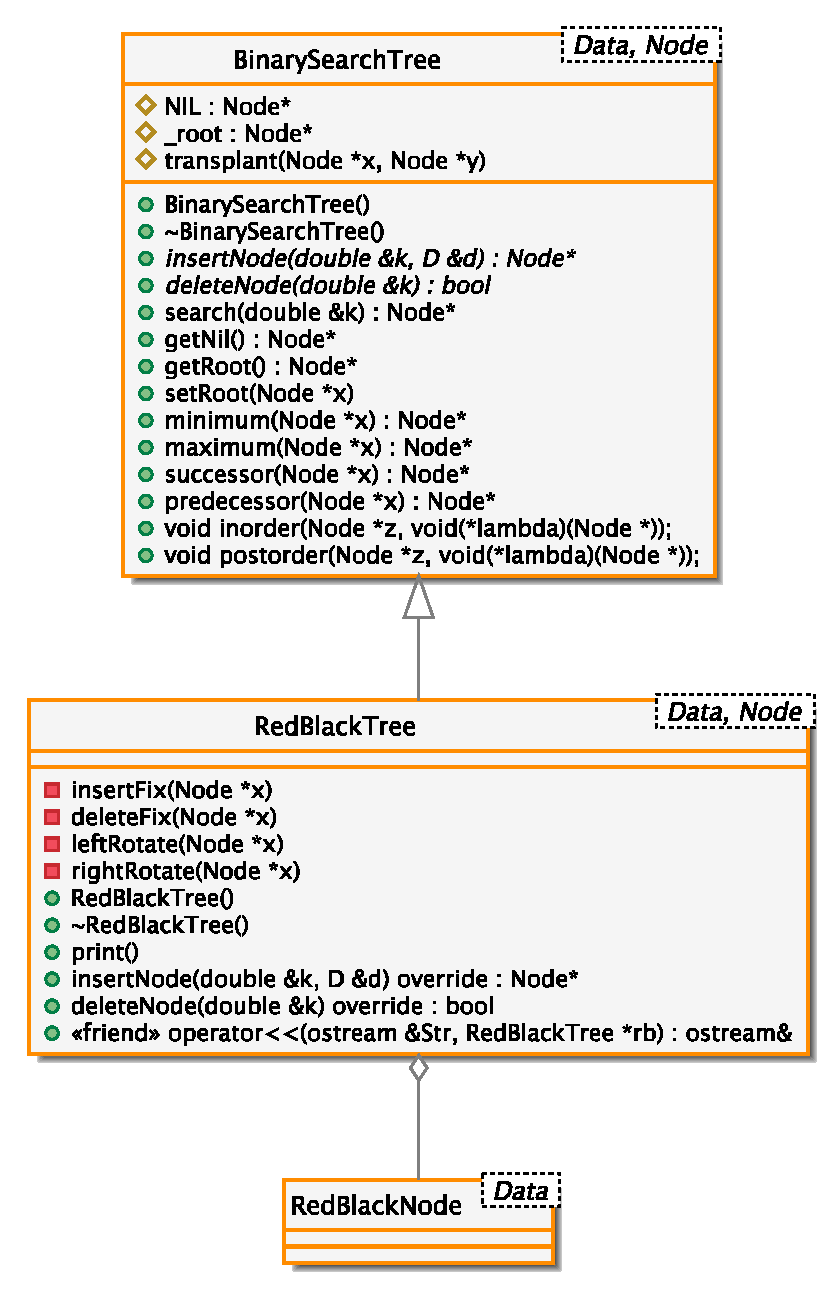
\includegraphics[scale=0.7]{src/rbhash/2img/trees.eps}
\captionof{figure}{Alberi}
\end{center}
\subsection{Hash Table}
Onde evitare di dover riscrivere codice si \`e scelto di sfruttare
il nodo generico anche per l'\textbf{HashTable}. A tal proposito
si \`e sviluppato una tabella hash ad \textbf{indirizzamento aperto} che
prende in input come paramentro templato, il dato da conservare.
Per risolvere le collisioni si \`e scelto di usare due funzioni hash:
\texttt{k} \`e un valore double che indica
la chiave, $\texttt{i}$ \`e l'iteratore che al massimo 
$\texttt{m}$ volte \footnote{m \`e il size dell'hashtable}  
applicher\`a la funzione di hash. La prima restituisce un indice con valore compreso
tra $[0, m]$, mentre la seconda funzione di hash un valore compreso tra $[1, m-1]$. 
Verr\`a usata la prima funzione di hash e in caso di collisione
si riapplicher\`a
$h(i, m) = (h_1(k) + i * h_2(k)) \ mod \ m$. Sebbene con un costo 
computazionale pi\`u alto, il doppio hashing risolve le collisioni
pi\`u in fretta rispetto allispezione lineare o quadratica.\newline \indent 
La funzione $search()$ nella class \textbf{HashTable}
\`e stata sovraccaricata per restituire valori diversi. Con la 
ricerca per valore si restituise, se disponibile un indice che 
usato nella seconda funzione di ricerca restituisce il dato.

\begin{center}
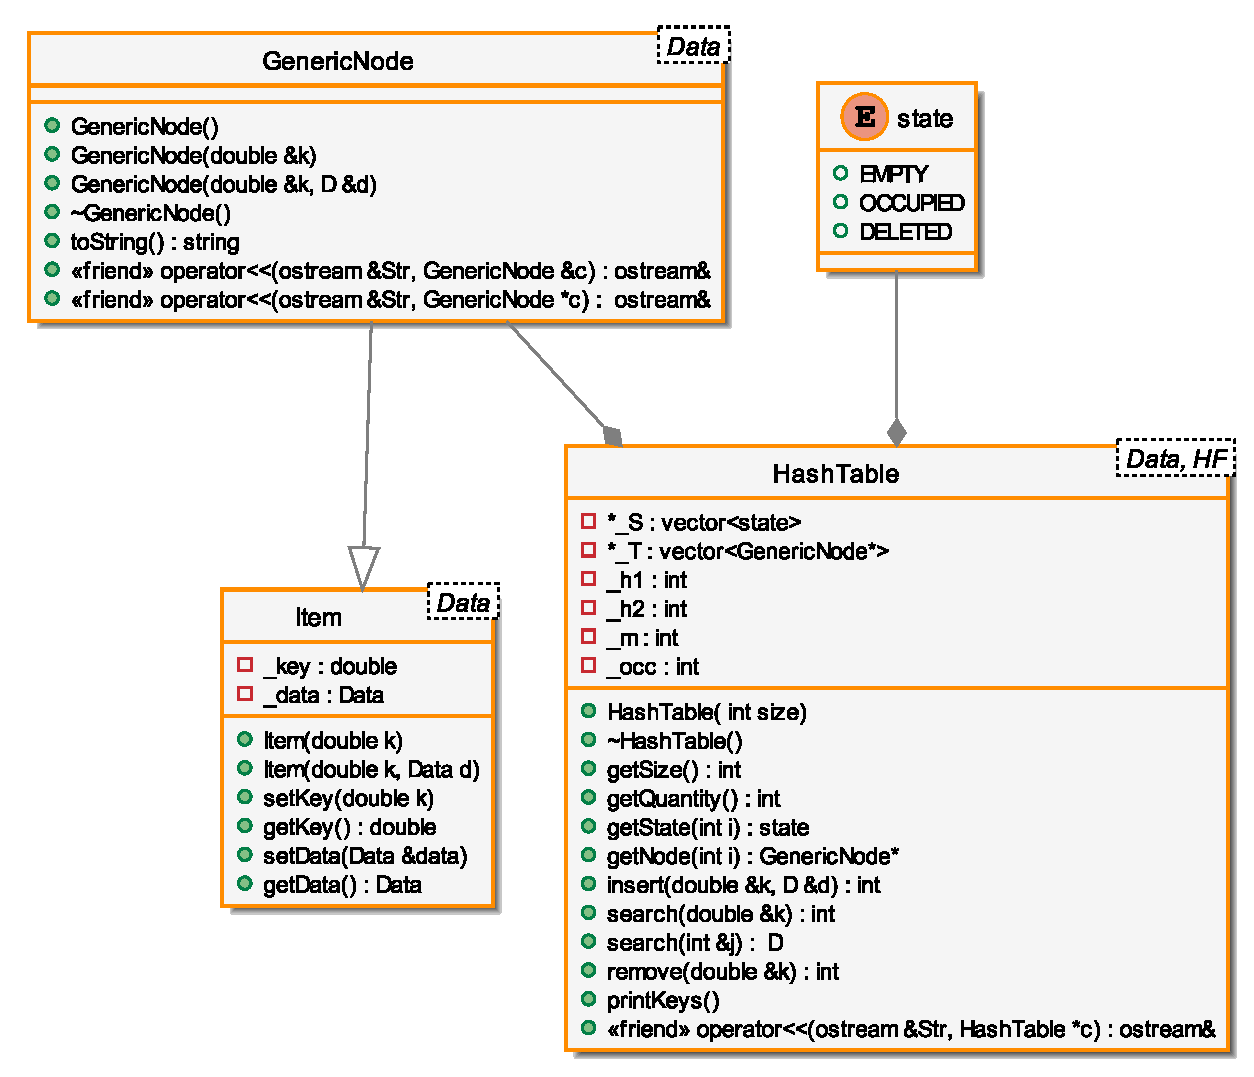
\includegraphics[scale=0.7]{src/rbhash/2img/hash.eps}
\captionof{figure}{Hash Table}
\end{center}

\newpage
\subsection{Red Black Hash}
La struttura dati realizzata fa uso degli alberi red black
e delle tavole di hash come spiegato nel primo paragrafo.
Si è scelto di usare una classe \textbf{Parser} per riempire la
struttura dati delle tuple contenute nel file di testo
o di quelle inserite tramite riga di comando.
\begin{center}
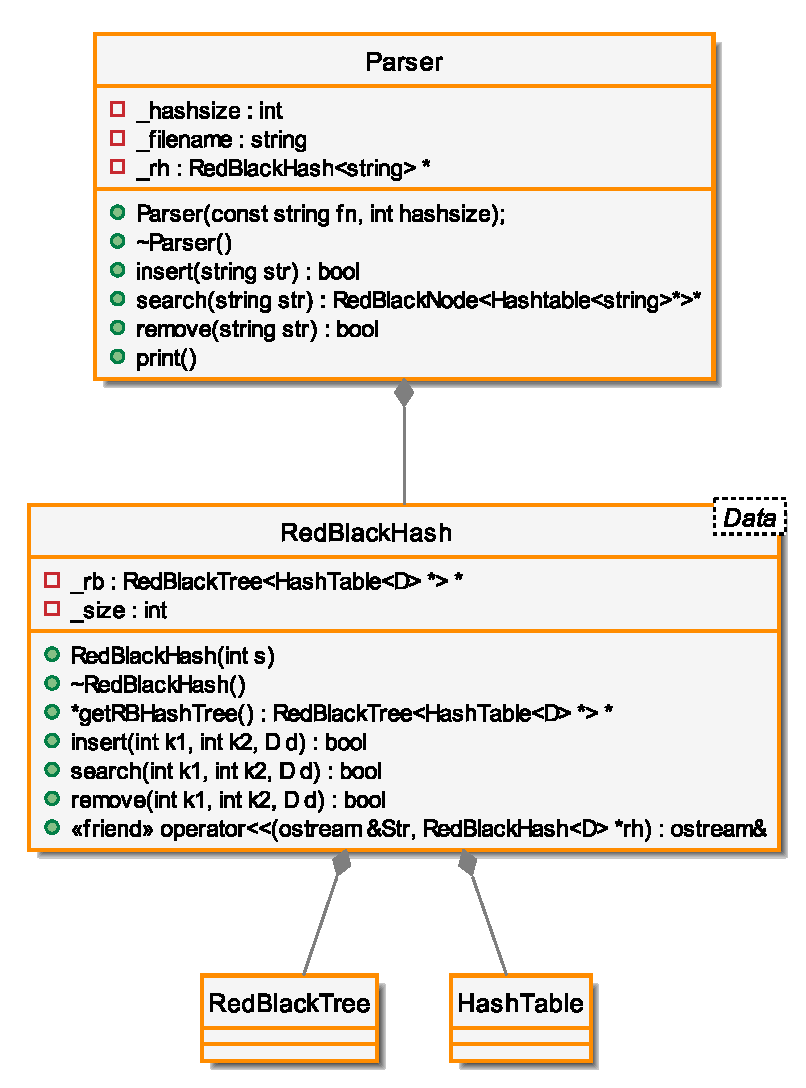
\includegraphics[scale=0.8]{src/rbhash/2img/rbhash.eps}
\captionof{figure}{Parser e RBH}
\end{center}\newpage
\def\baselinestretch{1}
\section{Studio complessit\`a}
\def\baselinestretch{1.66}
\thispagestyle{headings}
\indent Come detto precedentemente gli alberi Red Black hanno una complessit\`a temporale
nel \textbf{caso peggiore} al pi\`u equivalente ad $O(log_2 n)$ poich\'e bisogna scorrere tutto
l'albero in profondit\`a.\newline

\indent Le tabelle di hash a indirizzamento aperto, con doppia funzione di hash hanno complessit\`a temporali
prossime all'\textit{hashing 'ideale'}. Per poter assicurare che le due funzioni di hash producano
complessit\`a nel caso medio uguali a $O(1)$, si deve scegliere un valore della tavola di hash uguale ad
un numero primo o come potenza di due, e usare la seconda funzione di hash (quella che scandisce l'offset
dato dalle ispezioni successive) con un valore poco pi\`u piccolo di $m$ ($m-1$ o $m-2$).
In tal modo il doppio hashing usa $O(m^2)$ sequenze di ispezione,
perch\'e ogni coppia ($h_1(k), h_2(k)$) produce una distinta sequenza di ispezione.
Le \textbf{hashtable nel caso migliore}, ovvero non avendo nessuna collisione inseriscono,
cercano e cancellano i dati in $O(1)$.
Nel caso \textbf{peggiore} avremo un tempo massimo di $O(m)$,
dovuto alla scansione lineare di tutta la tavola di hash: ci\`o \`e  dovuto alla hashtable che si riempie
cio\`e quando il \textbf{ fattore di carico} (rapporto di elementi
inseriti e size della tavola) $\alpha$ tende a $1$.\newline

\indent Nella struttura dati \textbf{red-black hash} quando effettuiamo un \textbf{inserimento} andremo prima
ad effettuare una ricerca nell'albero rosso nero ($O(log_2n)$):
\begin{itemize}
    \item se esiste il nodo di chiave 1 allora
effettuiamo una ricerca nell'hash table tramite la chiave 2, e se possibile concludiamo l'inserimento.
Nel caso medio avremo una complessit\`a del tipo
$O(log_2n) + O(1) + O(1)$ e $O(log_2n) + O(m) + O(m)$ se l'hashtable ha un fattore di carico prossimo
all'1. In altri termini $\mathbf{O(log_2n)}$ e $\mathbf{O(m+log_2n)}$.;
    \item se invece il nodo di chiave 1 non esiste, dobbiamo allocare una hashtable, mappare la stringa alla chiave 2
e inserirla nell'albero: ci\`o porta una complessit\`a pari a $O(log_2n) + O(1) +  O(log_2n)$ ovvero 
$\mathbf{O(log_2n)}$.
\end{itemize}
L'operazione di \textbf{ricerca} impiega $\mathbf{O(m+log_2n)}$ nel caso in cui esista il nodo
con chiave 1 e la ricerca nella tavola hash restituisca l'indice in un tempo lineare; l'uso di tale indice 
serve per accedere al dato in $O(1)$. Nel caso migliore invece la ricerca avviene in
$\mathbf{O(log_2n)}$.\newline
La \textbf{cancellazione} ha complessit\`a uguali alle precendenti: si effettua una ricerca e
se l'hashtable ha solo un elemento allora si provvede a cancellare l'intero nodo dall'albero, altrimenti
si cancella solamente nell'hashtable: pertanto $\mathbf{O(log_2n)}$ oppure $\mathbf{O(m+log_2n)}$.
\newline
Tramite questo prospetto possiamo affermare che i casi peggiori sono dettati dalla tavola di hash e dipende
tutto dal suo fattore di carico.\newpage
\def\baselinestretch{1}
\section{Test e risultati}
\def\baselinestretch{1.66}
\thispagestyle{headings}

\subsection{Test effettuati}\newpage
\def\baselinestretch{1}
\section{Codice sorgente}
\def\baselinestretch{1.66}
\thispagestyle{headings}

\inputminted
[fontsize=\small,baselinestretch=1,
frame=lines,
framesep=10pt,
linenos=true,tabsize=2,
breaklines=true]{c++}{tesina_tex/source/graph/heap.hpp}
\inputminted
[fontsize=\small,baselinestretch=1,
frame=lines,
framesep=10pt,
linenos=true,tabsize=2,
breaklines=true]{c++}{tesina_tex/source/graph/heap.cpp}

\newpage
\inputminted
[fontsize=\small,baselinestretch=1,
frame=lines,
framesep=10pt,
linenos=true,tabsize=2,
breaklines=true]{c++}{tesina_tex/source/graph/minHeap.hpp}
\inputminted
[fontsize=\small,baselinestretch=1,
frame=lines,
framesep=10pt,
linenos=true,tabsize=2,
breaklines=true]{c++}{tesina_tex/source/graph/minHeap.cpp}
\newpage
\inputminted
[fontsize=\small,baselinestretch=1,
frame=lines,
framesep=10pt,
linenos=true,tabsize=2,
breaklines=true]{c++}{tesina_tex/source/graph/minPriorityQueue.hpp}
\inputminted
[fontsize=\small,baselinestretch=1,
frame=lines,
framesep=10pt,
linenos=true,tabsize=2,
breaklines=true]{c++}{tesina_tex/source/graph/minPriorityQueue.cpp}
\newpage


\inputminted
[fontsize=\small,baselinestretch=1,
frame=lines,
framesep=10pt,
linenos=true,tabsize=2,
breaklines=true]{c++}{tesina_tex/source/graph/galacticgraph.hpp}
\inputminted
[fontsize=\small,baselinestretch=1,
frame=lines,
framesep=10pt,
linenos=true,tabsize=2,
breaklines=true]{c++}{tesina_tex/source/graph/galacticgraph.cpp}
\newpage

\inputminted
[fontsize=\small,baselinestretch=1,
frame=lines,
framesep=10pt,
linenos=true,tabsize=2,
breaklines=true]{c++}{tesina_tex/source/graph/loader.hpp}
\inputminted
[fontsize=\small,baselinestretch=1,
frame=lines,
framesep=10pt,
linenos=true,tabsize=2,
breaklines=true]{c++}{tesina_tex/source/graph/loader.cpp}
\newpage

\inputminted
[fontsize=\small,baselinestretch=1,
frame=lines,
framesep=10pt,
linenos=true,tabsize=2,
breaklines=true]{c++}{tesina_tex/source/graph/debug.hpp}
\inputminted
[fontsize=\small,baselinestretch=1,
frame=lines,
framesep=10pt,
linenos=true,tabsize=2,
breaklines=true]{c++}{tesina_tex/source/graph/item.hpp}
\newpage

\inputminted
[fontsize=\small,baselinestretch=1,
frame=lines,
framesep=10pt,
linenos=true,tabsize=2,
breaklines=true]{c++}{tesina_tex/source/graph/vertex.hpp}
\inputminted
[fontsize=\small,baselinestretch=1,
frame=lines,
framesep=10pt,
linenos=true,tabsize=2,
breaklines=true]{c++}{tesina_tex/source/graph/vertex.cpp}
\newpage

\inputminted
[fontsize=\small,baselinestretch=1,
frame=lines,
framesep=10pt,
linenos=true,tabsize=2,
breaklines=true]{c++}{tesina_tex/source/graph/graph.hpp}
\inputminted
[fontsize=\small,baselinestretch=1,
frame=lines,
framesep=10pt,
linenos=true,tabsize=2,
breaklines=true]{c++}{tesina_tex/source/graph/graph.cpp}
\newpage\newpage
\newpage
\def\baselinestretch{1}
\begin{thebibliography}{30}
\bibitem{Cormen}
\textit{Introduzione agli algoritmi e strutture dati (Italiano), 2010}\\
Thomas H. Cormen (Autore),
Charles E. Leiserson (Autore),
Ronald L. Rivest (Autore),
Clifford Stein (Autore),
L. Colussi (a cura di).
\bibitem{SLIDE} Slide del corso \textit{Algoritmi e Strutture Dati e Laboratorio di Algoritmi e Strutture Dati}, tenuto dai docenti
\textit{F. Camastra e A. Ferone}.
\bibitem{OVERLEAF} Overleaf Documentation\\
\url{https://www.overleaf.com/learn/}
\bibitem{TEX} L'arte del \LaTeX, \textit{Lorenzo Pantieri}\\
\url{http://www.lorenzopantieri.net/LaTeX.html}
\bibitem{LISTING} \LaTeX/Source Code Listings\\
\url{https://en.wikibooks.org/wiki/LaTeX/Source_Code_Listings}
\bibitem{CRTP} Curiously recurring template pattern\\
\url{https://en.wikipedia.org/wiki/Curiously_recurring_template_pattern}
\bibitem{THECRTP} Curiously Recurring Template Pattern\\
\url{https://www.fluentcpp.com/2017/05/12/curiously-recurring-template-pattern/}
\end{thebibliography}
\newpage
    

\end{document}
